\chapter*{Введение} % * - чтобы не нумеровалось 
\addcontentsline{toc}{chapter}{ Введение}  % Но тогда надо в содержание... 

В настоящее время активно развивается рынок Web-приложений. Все больше различных услуг 
предоставляется через Интернет, классические информационные системы в различных компаниях
 также становятся Web-приложениями, предоставляя для своих сотрудников и партнеров 
 доступ к ресурсам компании не только из локальной, но и из глобальной сети. Концепции 
 и технологии,  используемые при разработке web-приложений, постоянно развиваются и 
 совершенствуются.  Оптимизируется использование ресурсов и времени, улучшаются 
 возможности по отображению предоставляемой информации,  динамичность и интерактивность
  web-приложений.

На сегодняшний день одним из наиболее перспективных подходов к обеспечению всего 
вышеперечисленного является концепция Rich Internet Application (в дальнейшем RIA) - 
это приложения, доступные через сеть Интернет, обладающие  особенностями и 
функциональностью традиционных настольных приложений.
 
Приложения RIA, как правило:

\begin{enumerate}

\item передают веб-клиенту необходимую часть пользовательского   интерфейса, 
оставляя большую часть данных (ресурсы программы, данные и пр.) на сервере;
\item запускаются в браузере  и не требуют дополнительной установки программного 
обеспечения;
\item запускаются локально в среде безопасности, называемой <<песочница>>(sandbox).
\end{enumerate}

На Рис.~\ref{ris:RIAinWorld.png} демонстрируется место Rich Internet Applications 
среди других технологий программных систем
\begin{figure}[h]
\center{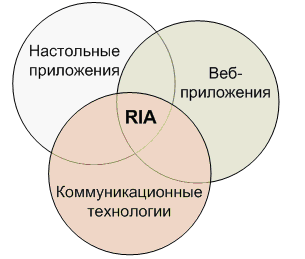
\includegraphics[height=60mm, width=80mm]{RIAinWorld.png}}
\caption{RIA среди других технологий}
\label{ris:RIAinWorld.png}
\end{figure}

Термин «RIA» впервые был упомянут компанией  Macromedia в официальном сообщении в 
марте 2002 года. Подобные концепции существовали и несколькими годами ранее, например:

\begin{enumerate}

\item DHTML;
\item X Internet (компания Forrester Research в 2000 году);
\item Rich (web) clients; 
\item Rich web application. 

\end{enumerate}

Для начала рассмотрим архитектурные особенности построения web-приложений базирующихся 
на RIA  концепции.  Для этого сравним принципработы традиционного web-приложения и 
RIA-приложения ( Рис.~\ref{ris:principlesRIA.png} ).  
\begin{figure}[h]
\center{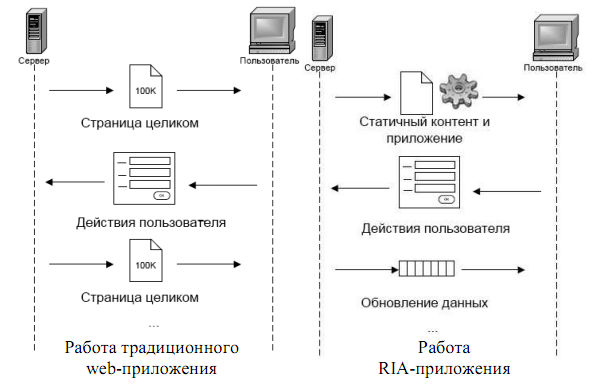
\includegraphics[height=80mm, width=100mm]{principlesRIA.png}}
\caption{Принципы работы традиционного web-приложения и RIA приложения}
\label{ris:principlesRIA.png}
\end{figure}

Работа традиционных web-приложений сконцентрирована вокруг клиент серверной архитектуры 
с тонким клиентом.  Такой клиент переносит все задачи по обработке информации на сервер, 
а сам используется в основном для отображения статического контента.  Основной 
недостаток этого подхода в том,  что все взаимодействие с приложением должно 
обрабатываться сервером,  что требует постоянной отправки данных на сервер,  
ожидания ответа сервера, и загрузки страницы обратно в браузер. В отличие от 
традиционного web-приложения в RIA  значительная часть функционала исполняется на 
стороне клиента,  поэтому появляется возможность отправлять и получать данные с сервера 
только по мере необходимости.  Если подключение нестабильно,  клиентская часть RIA- 
приложения обладает возможностями кэширования данных и работы без подключения к сети в 
режиме offline.

На основе вышесказанного, можно выделить ряд преимуществ RIA  как перед настольными приложения, 
так и перед стандартными веб-приложениями:

\begin{enumerate}

\item не требуется установка приложения – как правило, все что необходимо, это установка плагина 
для браузера;
\item обновление и распространение приложения  – быстрый и автоматизированный процесс;
\item пользователи могут использовать приложение на любом компьютере, имеющем соединение с Интернет, 
причем обычно не важно, какая операционная система на нем установлена;
\item интерфейс  RIA обладает большей интерактивностью, он не ограничен лишь использованием языка 
HTML, применяемого в стандартных веб-приложениях. Наиболее сложные приложения RIA предлагают 
внешний вид и функциональность, близкие к настольным приложениям;
\item При работе веб-приложения компьютер пользователя гораздо меньше подвержен вирусному заражению, 
чем при запуске исполняемых бинарных файлов
\item Использование вычислительных ресурсов клиента и сервера лучше сбалансировано;
\item Асинхронная коммуникация (взаимодействие клиента с сервером без ожидания каких-либодействий 
пользователя).

\end{enumerate}

Для реализации RIA многими IT-компаниями предлагаются различные технологии. Наиболее известными из 
них являются AJAX,  Flash, Flex (в дальнейшем Flex)  и AIR  фирмы Adobe; ActiveX, WPF  и Silverlight  
корпорации Microsoft; Java FX  и Java Applets  компании Sun Microsystems .

В настоящее время одной из наиболее распространенных технологий разработки RIA является Adobe Flex,  
которая представляет собой  среду с открытым кодом для создания и обслуживания web-приложений, 
совместимую со всеми распространенными браузерами,  платформами персональных компьютеров и версиями 
операционных систем и имеющую максимальную поддержку со стороны разработчиков. 

Flex представляет собой набор классов,  расширяющих возможности Flash. Flex позволяет описывать 
интерфейс web-приложения на MXML – декларативном языке описания и настройки свойств визуальных 
элементов интерфейса, основанном на XML. Логика web-приложения пишется на ActionScript –  полноценном 
объектно-ориентированном языке программирования,  который является одним из диалектов ECMAScript. 
Результатом компиляции является файл SWF,  предназначенный для выполнения в браузере (на платформе 
Flash Player,  которая существует в виде плагина к браузеру)  или как самостоятельное приложение (на 
платформе AIR).
  
Flex-framework включает возможности локализации, стилизации приложения, разработки модульного приложения, 
встроенные валидаторы и форматоры текстовых полей — все те инструменты, которые нужны разработчикам 
приложений, работающих online. Также Flex предоставляет полные мультимедийные возможности Flash 
Platform, такие как потоковое мультимедиа,  возможность получить доступ к веб-камере и микрофону 
пользователя, бинарные сокеты, обширные возможности сетевых коммуникаций (HTTP-запросы, веб-сервисы, 
встроенный формат сериализации AMF), оперирование координатами трехмерного пространства).

Вся разработка во Flex  ориентирована на применение готового набора
расширяемых компонентов,  внешний вид которых позволяет гибко
настраивать CSS, что облегчает задачу разработчика. 

Flex SDK  является бесплатным инструментарием с июня 2007 
года с открытым исходным кодом,  распространяемым на условиях Mozilla Public License.  
Для работы с процедурами и классами этого фреймворка можно использовать как бесплатные 
(Eclipse WTP IDE, FlashDevelop IDE) так и платные (Flex Builder IDE, IntelliJ IDEA IDE, 
Aptana Studio IDE, PowerFlasher FDT IDE) среды разработки.

Flex приложения предоставляют возможность реализации клиент-серверного взаимодействия 
на основе бинарного формата обмена данными - AMF(Action Message Format). AMF 
используется для сериализации структурированных данных, таких как объекты Action Script 
или XML, и обмена сообщениями между Adobe Flash клиентом и удалённым сервисом. 
AMF более экономичен по трафику по сравнению с XML и позволяет передавать типизированные объекты.

Однако использование AMF вызывает ряд трудностей для реализации автоматизации функционального 
и нагрузочного тестирования взаимодействия сервера и Flex клиента, связанных с бинарной 
природой протокола. Так как amf сообщение представляет собой совокупность байтов, 
разработчикам и тестировщикам трудно считывать и изменять содержащуюся в нём информацию.

Отдельной проблемой является нагрузочное тестирование таких приложений - имитация работы с 
приложением большого количества пользователей за счёт запуска набора тестов в несколько потоков. 
Сложность состоит в поддержке уникальности идентификатора сессии каждого клиента. Идентификатор 
клиента выделяется строго одному подключенному SWF- файлу и прошит в передаваемых данных. 
Стандартный порядок тестирования - запись запросов пользователя с использованием прокси-сервера 
и запуск сохранённого сценария в несколько потоков - в данном случае будет неэффективным, так 
как  все перехваченные запросы будут иметь одинаковый идентификатор клиента и тесты пройдут 
только в 1 потоке, а остальные будут возвращены с ошибкой о неправильной сессии.
 
Поиск решения проблемы автоматизации тестирования взаимодействия Flex приложений с сервером 
через протокол AMF и будет являться задачей моего дипломного проекта.
